
\(f(x) = (5 - 2x)\e^x\).

\subsection*{1.}

\begin{itemize}
    \item \(A\) d'abscisse nulle appartient à \(C\), son ordonnée est donc \(f(0) = 5\e^0 = 5\). Donc \(A(0\,;\,5)\).
    \item \(B\) d'ordonnée nulle appartient à \(C\), son abscisse est donc telle que :
    \[
    f(x) = 0 \quad \Longleftrightarrow \quad (5 - 2x)\e^x = 0 \quad \Longleftrightarrow \quad 5 - 2x = 0,
    \]
    puisqu'on sait que, quel que soit \(x\),  \(\e^x > 0\).
    
    Donc : \(5 = 2x \Longleftrightarrow x = \dfrac{5}{2}\) et \(B\left(\dfrac{5}{2}\,;\,0\right)\).
\end{itemize}

\subsection*{2.}

\(f\), produit de fonctions dérivables sur \(\mathbb{R}\), est dérivable sur \(\mathbb{R}\) et sur cet intervalle :
\[
f'(x) = -2 \e^x + (5 - 2x)\e^x = \e^x(-2 + 5 - 2x) = (3 - 2x)\e^x.
\]

\subsection*{3.}

\(f'(x)\) est donc du signe de \(3 - 2x\) :
\begin{align*}
&3 - 2x > 0 \\
\iff&  3 > 2x \\
\iff & \dfrac{3}{2} > x
\end{align*}
donc la fonction \(f\) est croissante sur \(\left]-\infty\,;\,\dfrac{3}{2}\right[\) ;
	\begin{center}
	\begin{tikzpicture}[double distance=2pt]
		\tkzTabInit{$x$/1,f'(x)/1,$f(x)$/2}{$0$,$\dfrac{3}{2}$, $10$}
		\tkzTabLine{,+,z, -}
		\tkzTabVar{+/$0$,-/ $6\e^{-1}$ /, +/}
	\end{tikzpicture}
\end{center} 

\subsection*{4.}

D'après le résultat précédent \(D\left(1,5\,;\,2 e^{1,5}\right)\).

\subsection*{5.}

Une équation de la tangente \(T\) à la courbe \(C\) au point \(A\) d'abscisse \(0\) est :

\[
M(x\,;\,y) \in \mathcal T \quad \Longleftrightarrow \quad y - f(0) = f'(0)(x - 0).
\]

Avec \(f(0) = 5\) et \(f'(0) = 3\), on obtient :
\[
M(x\,;\,y) \in \mathcal T \quad \iff \quad y - 5 = 3x \quad \iff \quad y = 3x + 5.
\]

Or $D\left(1,5\,;\,2 \e^{1,5}\right) \in \mathcal T \iff 2\e^{1,5} = 4,5 + 5 $\\
Comme $ 2 \e^{1,5} \neq 9,5$ , alors $ D \notin \mathcal T$.

